\documentclass[11pt]{article}
	\usepackage[T1]{fontenc}
    % Nicer default font (+ math font) than Computer Modern for most use cases
    % \usepackage{mathpazo}

    % Basic figure setup, for now with no caption control since it's done
    % automatically by Pandoc (which extracts ![](path) syntax from Markdown).
    \usepackage{graphics}
    % We will generate all images so they have a width \maxwidth. This means
    % that they will get their normal width if they fit onto the page, but
    % are scaled down if they would overflow the margins.
    \makeatletter
    \def\maxwidth{\ifdim\Gin@nat@width>\linewidth\linewidth
    \else\Gin@nat@width\fi}
    \makeatother
    \let\Oldincludegraphics\includegraphics
    % Set max figure width to be 80% of text width, for now hardcoded.
    \renewcommand{\includegraphics}[1]{\Oldincludegraphics[width=.8\maxwidth]{#1}}
    % Ensure that by default, figures have no caption (until we provide a
    % proper Figure object with a Caption API and a way to capture that
    % in the conversion process - todo).
    \usepackage[center,bf]{caption}
    % \DeclareCaptionLabelFormat{nolabel}{}
    % \captionsetup{labelformat=nolabel}

    \usepackage{adjustbox} % Used to constrain images to a maximum size 
    \usepackage{xcolor} % Allow colors to be defined
    \usepackage{enumerate} % Needed for markdown enumerations to work
    \usepackage{geometry} % Used to adjust the document margins
    \usepackage{amsmath} % Equations
    \usepackage{amssymb} % Equations
    \usepackage{textcomp} % defines textquotesingle
    % Hack from http://tex.stackexchange.com/a/47451/13684:
    \AtBeginDocument{%
        \def\PYZsq{\textquotesingle}% Upright quotes in Pygmentized code
    }
    \usepackage{upquote} % Upright quotes for verbatim code
    \usepackage{eurosym} % defines \euro
    \usepackage[mathletters]{ucs} % Extended unicode (utf-8) support
    \usepackage[utf8x]{inputenc} % Allow utf-8 characters in the tex document
    \usepackage{fancyvrb} % verbatim replacement that allows latex
    \usepackage{grffile} % extends the file name processing of package graphics 
                         % to support a larger range 
    % The hyperref package gives us a pdf with properly built
    % internal navigation ('pdf bookmarks' for the table of contents,
    % internal cross-reference links, web links for URLs, etc.)
    \usepackage{hyperref}
    \usepackage{longtable} % longtable support required by pandoc >1.10
    \usepackage{booktabs}  % table support for pandoc > 1.12.2
    \usepackage[inline]{enumitem} % IRkernel/repr support (it uses the enumerate* environment)
    \usepackage[normalem]{ulem} % ulem is needed to support strikethroughs (\sout)
                                % normalem makes italics be italics, not underlines
   	\usepackage[]{authblk}
   	\usepackage{cite}
    \usepackage{graphicx}
    \usepackage{hyperref}
    \usepackage{amsmath}
    \usepackage{amsthm}
    \usepackage{amssymb}
    \usepackage{bm}
    \usepackage{bbm}
    \usepackage{algorithmicx}
    \usepackage{algorithm}
    \usepackage{algpseudocode}
    \usepackage{array}
    \usepackage{booktabs}
    \usepackage{multirow}
    \usepackage{makecell}
    \usepackage{color}
    \usepackage{tabularx,ragged2e,booktabs,caption}
    \usepackage{verbatim}
   	\makeatletter
    \def\@maketitle{%
    \newpage
      \null
      \vskip 2em%
      \begin{center}%
      \let \footnote \thanks
        {\Large\bfseries \@title \par}%
        \vskip 1.5em%
        {\normalsize
          \lineskip .5em%
          \begin{tabular}[t]{c}%
            \@author
          \end{tabular}\par}%
        \vskip 1em%
        {\normalsize \@date}%
      \end{center}%
      \par
      \vskip 1.5em}
    \makeatother


\newtheorem{theorem}{Theorem}






\title{EE 232E Project 5\\Graph Algorithms}
\author{Hengjie~Yang, Sheng~Chang, Wandi~Cui, and Tianyi~Liu
}


\date{\today}


\begin{document}
\maketitle


\begin{comment}
\section{A brief tutorial on how to use this template}
\Large\textcolor{red}{\bf{Please remove the tutorial section in the final manuscript\\ by commenting, i.e. $\%(something)$}}


\subsection{Figures}
Figure insertion is shown in Fig \ref{example_fig}.
\begin{figure}[h]
\centering
\scalebox{0.7}{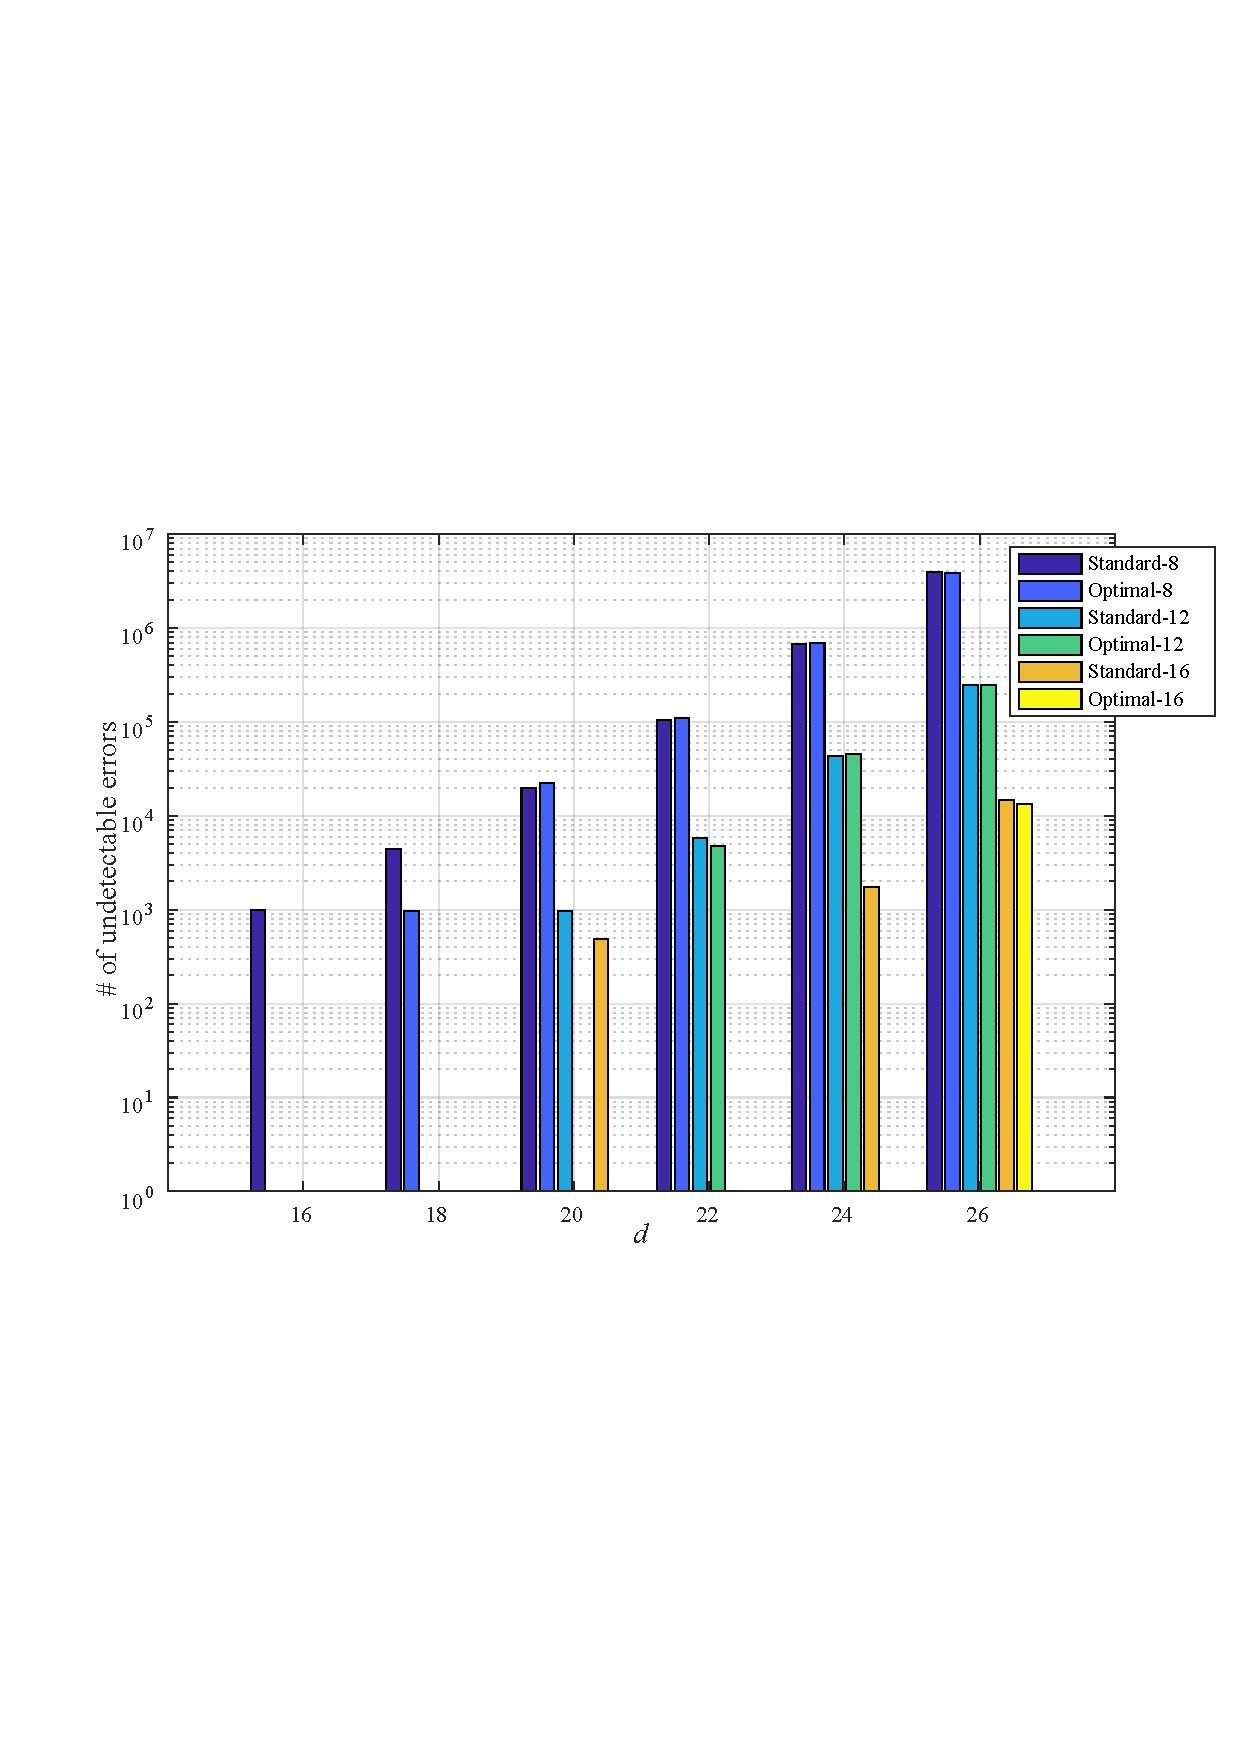
\includegraphics{Figures/spectrum_bar.pdf}}
\caption{An example of figure insertion}
\label{example_fig}
\end{figure}

\subsection{Equations}
An example of equations is given as follows.
\begin{theorem}
Let $a$, $b$, $c$ denote the sides of a triangle, respectively. If $a\perp b$, the pythagoras theorem is given as follows.
\begin{align}
c^2 = a^2 + b^2
\end{align}
\end{theorem}

\subsection{Tables}
An example of tables is shown in Table \ref{example_table}.
\renewcommand\arraystretch{1.1}
\begin{table}[h]
\center
\caption{Standard CRC Codes versus Optimal CRC Codes for Convolutional Code $G=(561~753)$ with $n=504$ Bits}
\scalebox{0.9}{
\begin{tabular}{r|c|c|cccccc}
\hline
\multirow{2}{*}{Name} & \multirow{2}{*}{Gen. Poly.} & \multicolumn{7}{c}{Undetected Error Distance Spectrum} \\
\cline{3-9}
 & & $d$ & 16 & 18 & 20 & 22 & 24 & 26 \\\hline\hline
Standard-8 & \multicolumn{1}{l}{0x19B} & & 983 & 4387 & 19909 & 105000 & 672724 & 3972970\\
Optimal-8 & \multicolumn{1}{l}{0x19D} & & 0 & 979 & 22349 & 111304 & 686314 & 3830340\\\hline
Standard-12 & \multicolumn{1}{l}{0x180F} & & 0 & 0 & 969 & 5815 & 42893 & 245211 \\
Optimal-12 & \multicolumn{1}{l}{0x108B} & & 0 & 0 & 0 & 4793 & 45795 & 246729\\\hline
Standard-16 & \multicolumn{1}{l}{0x11021} & & 0 & 0 & 484 & 0 & 1765 & 14752\\
Optimal-16 & \multicolumn{1}{l}{0x1F8FD} & & 0 & 0 & 0 & 0 & 0 & 13240\\\hline
\end{tabular}}
\label{example_table}
\end{table}

 \end{comment}

\section{Stock Market}

\subsection{Return Correlation}
\textcolor{blue}{Question 1: Provide an upper and lower bound on $\rho_{ij}$. Also, provide a justification for using log-normalized return $r_i(t)$ instead of regular return $q_i(t)$.}

According to the formula of $\rho_{ij}$, the upper bound should be $1$ and the lower bound should be $-1$, where $r_i(t) = r_j(t)$ and $r_i(t) = -r_j(t)$ respectively.

Considering the reason why we use log-normalized return $r_i(t)$ instead of regular return $q_i(t)$, we have following analysis and explanations:

\textbf{(a)log-normality:} if we assume that prices are distributed log normally (which, in practice, depends on the given price series), then $r_i(t)$ is conveniently normally distributed, because:
\begin{displaymath}r_i(t) = \log(1 + q_i(t)) = \log\frac{p_i(t)}{p_i(t-1)}\end{displaymath}
This is handy given much of classic statistics presumes normality.

\textbf{(b)Approximate raw-log equality:} when returns are very small (common for trades with short holding durations), the following approximation ensures they are close in value to raw returns:
\begin{displaymath}r_i(t) = \log(1 + q_i(t)) \approx q_i(t), where q_i(t)\ll 1\end{displaymath}

\textbf{(c)time-additivity:} Consider a stock $i$ with an ordered sequence of $n$ trades. A statistic frequently calculated from this sequence is the compounding return, which is the running return of this sequence of trades over time:
\begin{displaymath}q_i(1) \cdot q_i(2) \cdot q_i(3) \cdot...\cdot q_i(n)\end{displaymath}
This formula seems really complicated since the product of normally-distributed variables is not normal. Instead, the sum of normally-distributed variables is normal. This can show another benefit of representing returns in log-normality:
\begin{displaymath}r_i(1) + r_i(2) + r_i(3) + ... + r_i(n) =\log p_i(n) - \log p_i(0)\end{displaymath}
Thus, the compound return over $n$ periods is merely the difference in $log$ between initial and final periods. In terms of algorithmic complexity, this simplification reduces $O(n)$ multiplications to $O(1)$ additions. 

\textbf{(d)For Mathematical Ease:}
from calculus, we are reminded (ignoring the constant of integration):
\begin{displaymath}e^x = \int e^xdx = \frac{d}{dx} e^x = e^x\end{displaymath}

This identity is tremendously useful, as much of financial mathematics is built on continuous time stochastic processes which rely heavily on integration and differentiation.

\textbf{(e)Numerical stability:}
Sometimes the addition of small numbers is numerically safe, while multiplying small numbers is not as it is subject to arithmetic underflow. 

\subsection{Constructing Correlation Graphs}
\textcolor{blue}{Question 2: Plot the degree distribution of the correlation graph and a histogram showing the un-normalized distribution of edge weights.}

After constructing the correlation graph, the degree distribution we get is shown in Figure\ref {fig:Q2_1}
Not surprisingly, all vertices are connected with each other, so the degree of them are the same, equals to the number of vertices minus 1.

\begin{figure}[h]
\centering
\scalebox{0.7}{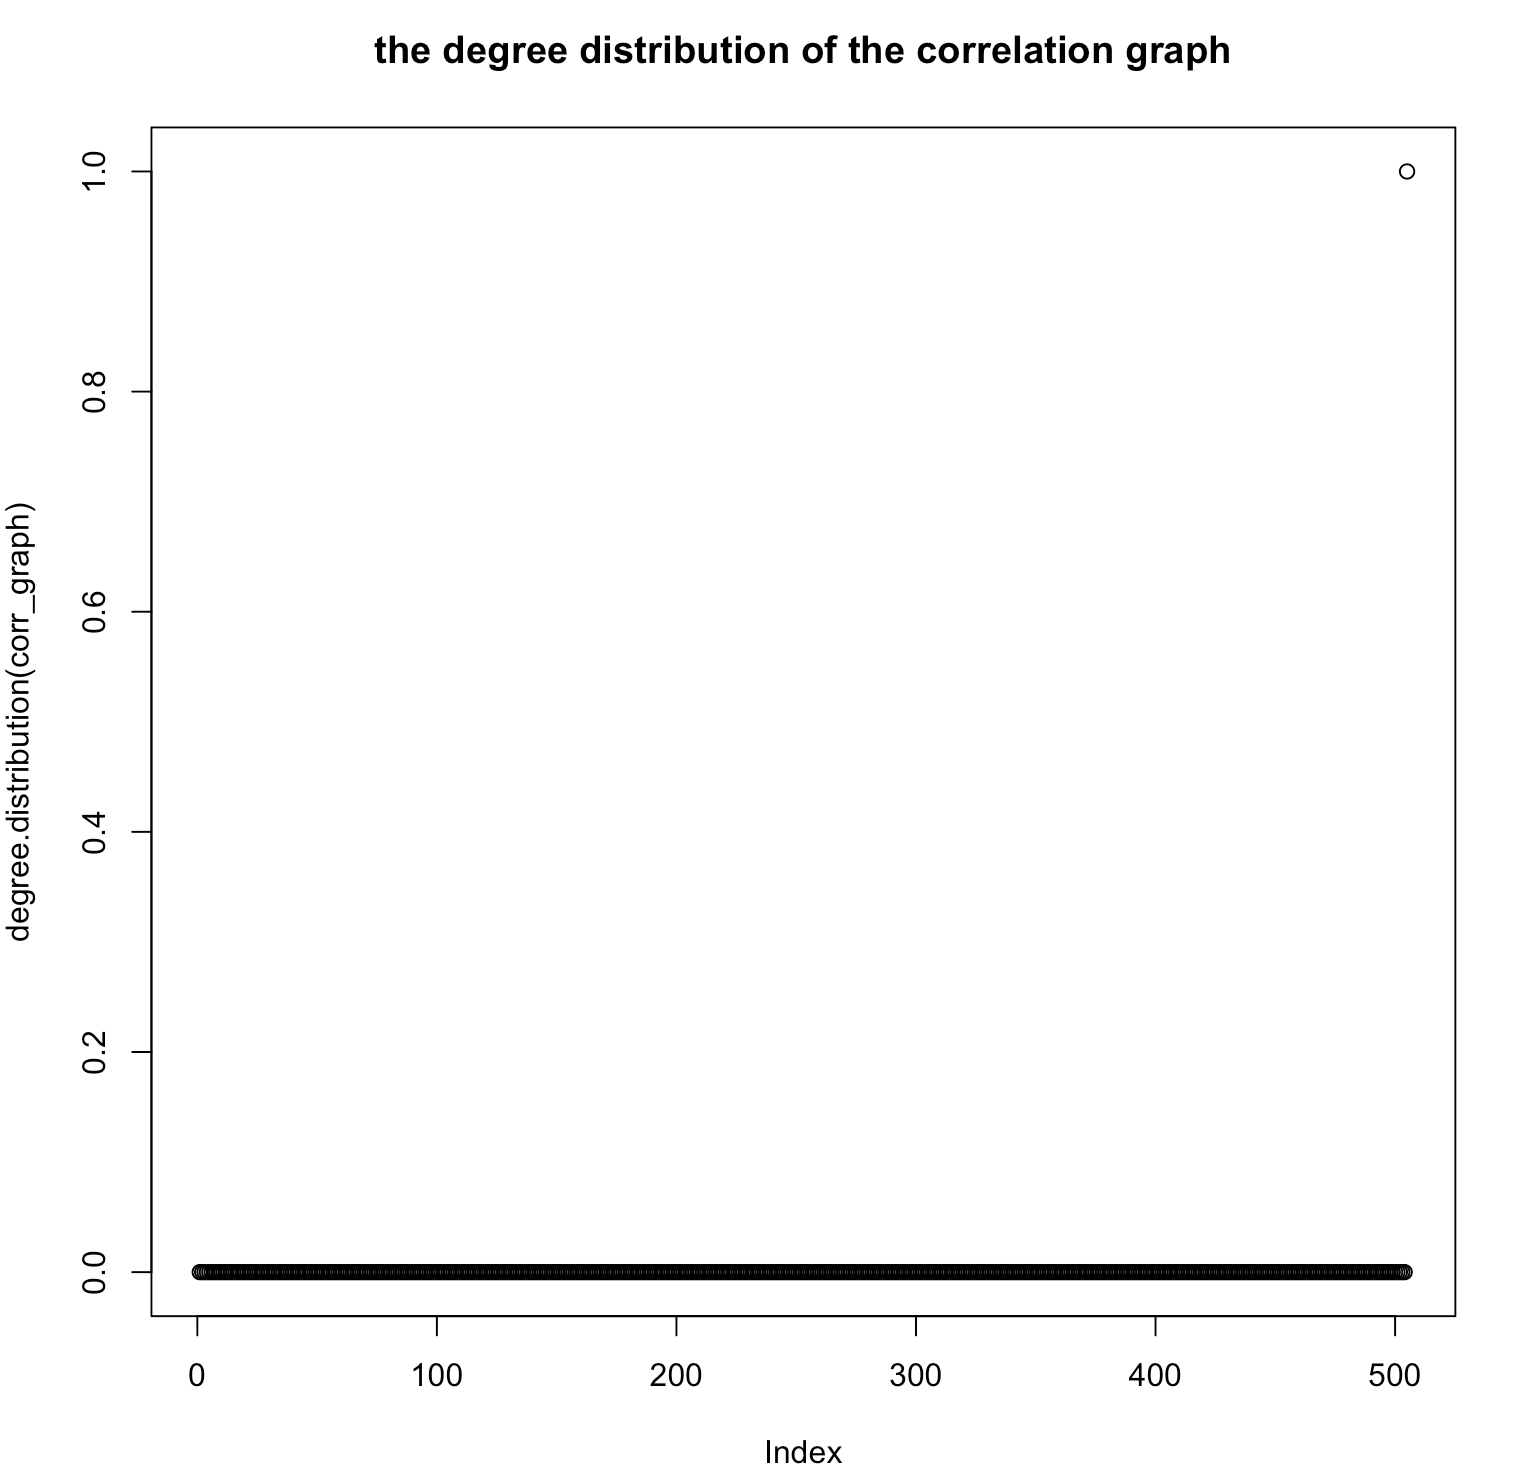
\includegraphics{Figures/degree_distribution.png}}
\caption{degree distribution of the correlation graph}
\label{fig:Q2_1}
\end{figure}

The edge weights distribution is shown in Figure\ref {fig:Q2_2}

\begin{figure}[h]
\centering
\scalebox{0.7}{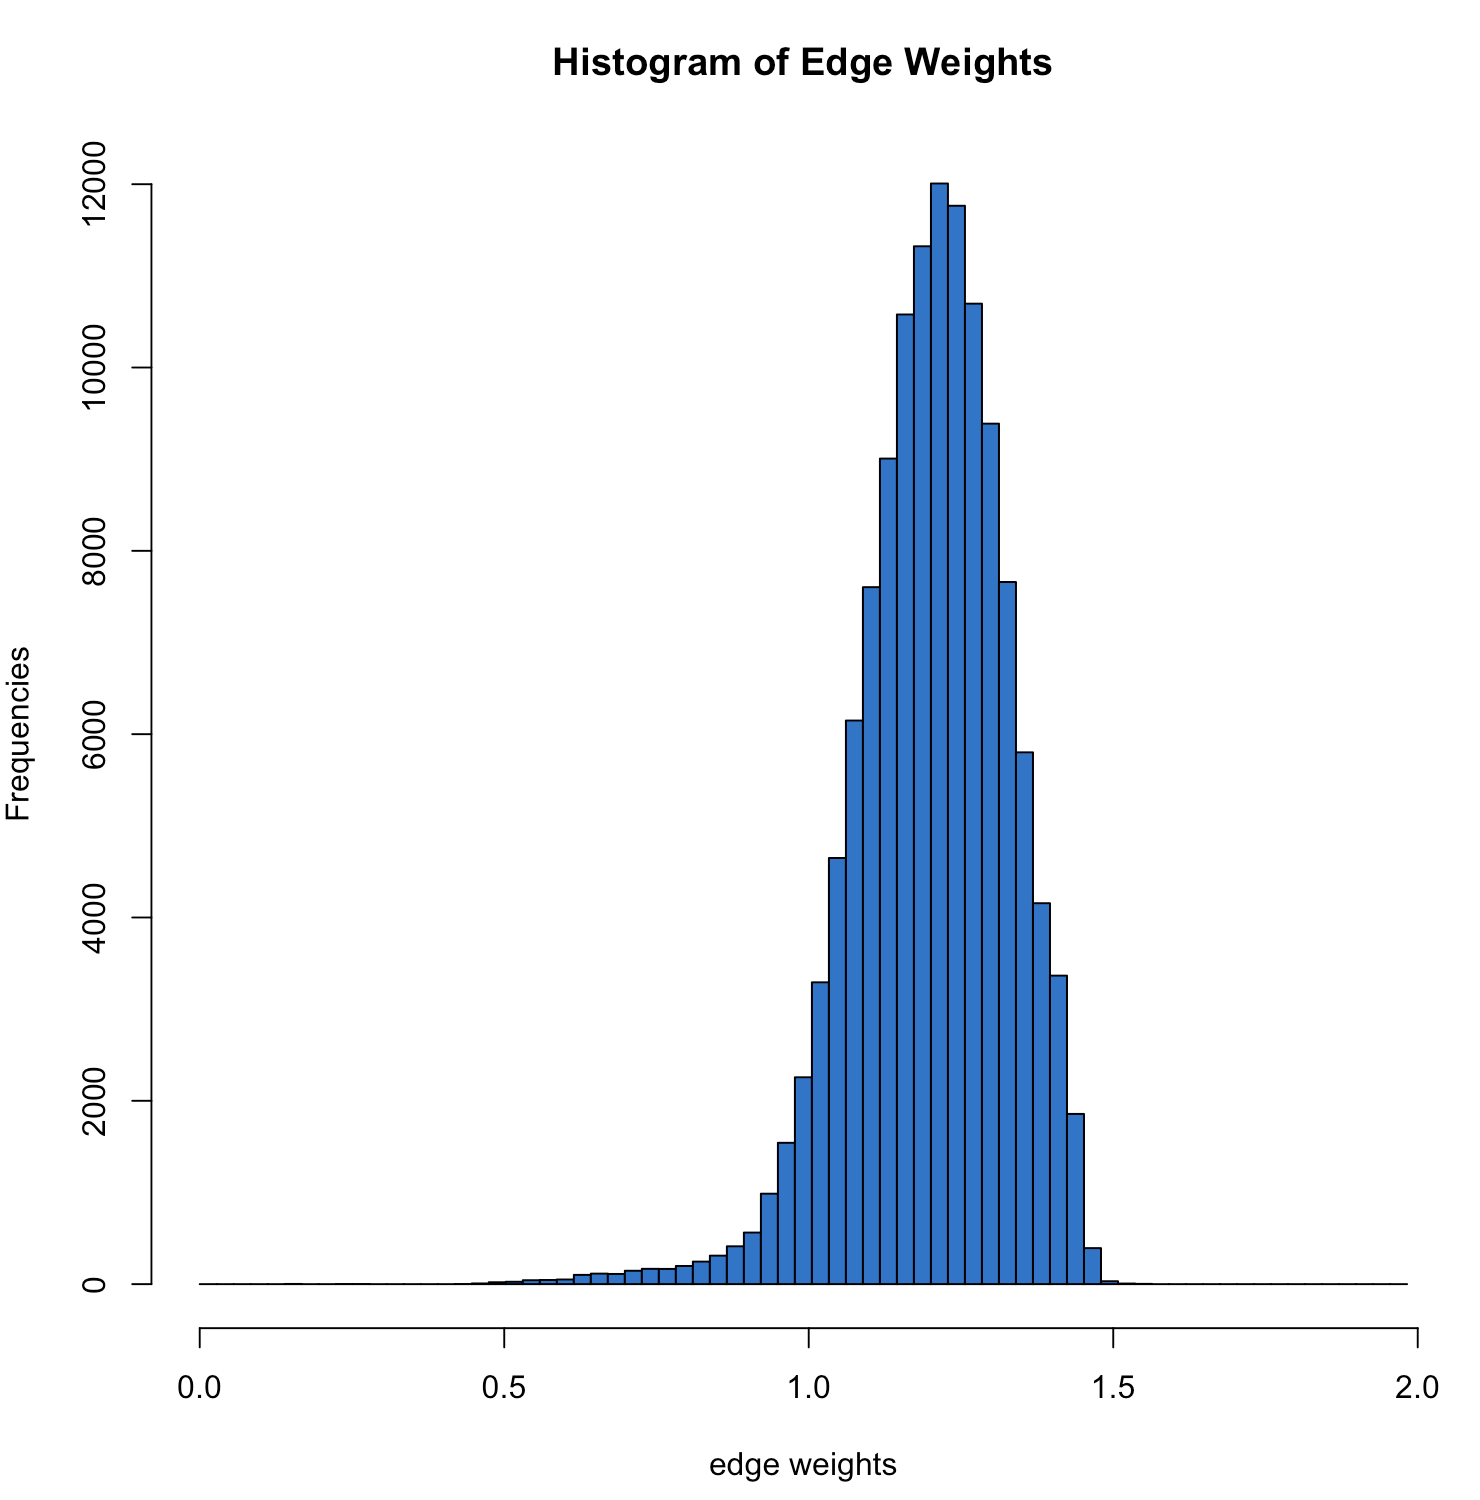
\includegraphics{Figures/edge_distribution.png}}
\caption{edge weights distribution of the correlation graph}
\label{fig:Q2_2}
\end{figure}

\subsection{Minimum Spanning Tree (MST)}
\textcolor{blue}{Question 3: Extract the MST of the correlation graph. Each stock can be categorized into a sector, which can be found in Name\_sector.csv file. Plot the MST and color-code the nodes based on sectors. Do you see any pattern in the MST? The structures that you find in MST are called Vine clusters. Provide a detailed explanation about the pattern you observe.
}

The MST plot is shown in Figure\ref {fig:Q3}, and differnt color represents different sectors of the stock.

We found that there is an interesting pattern in MST: stocks in same sector tend to be clustered together, and the whole MST looks like a grape-shaped graph. In fact, this is understandable, since the weight of the edge represents the correlation of the stock. It is not difficult to imagine that stocks are highly correlated so the weight between them is likely to be comparablly smaller than the weight between stocks in different sectors. Since MST find the path containing all the vertices in the graph with minimum total cost, it is reasonable to traverse nearly all the vertices in one sector and than transfer to another. That is why the pattern of MST looks like several "sector clusters" hanging in the tree, which is called "vine clusters" structure.
\begin{figure}[h]
\centering
\scalebox{0.7}{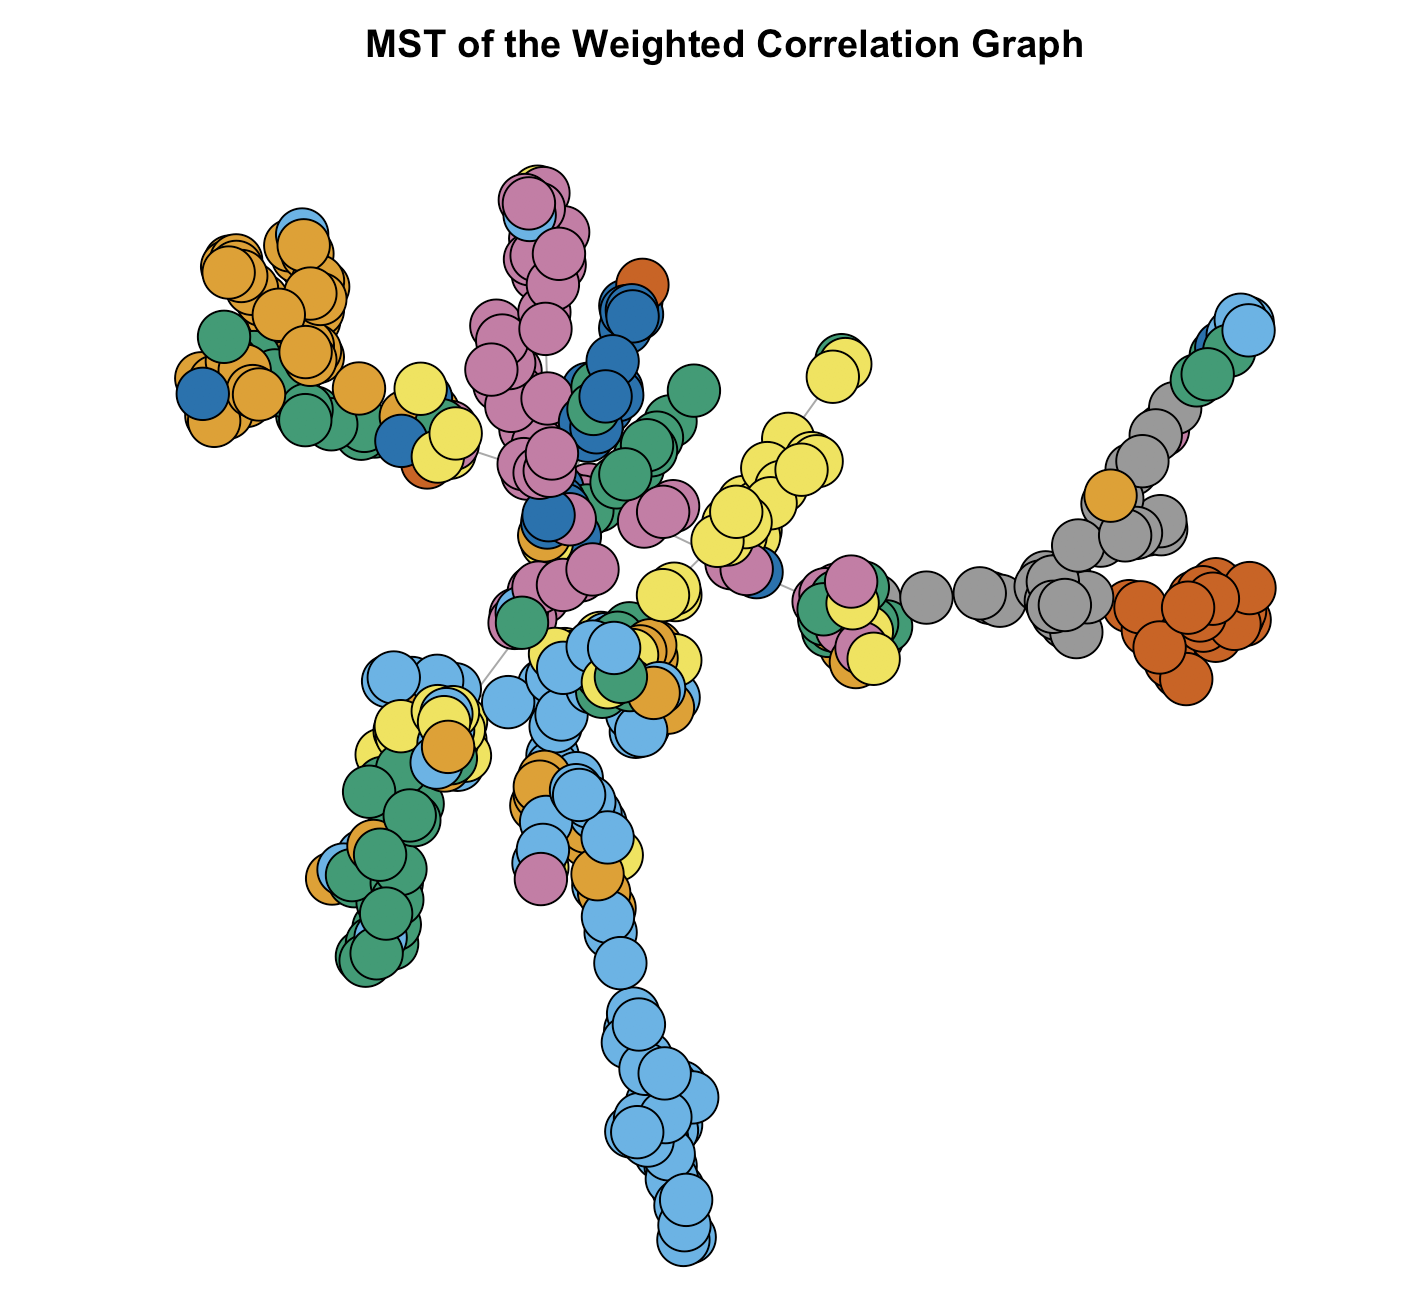
\includegraphics{Figures/MST.png}}
\caption{MST of the correlation graph}
\label{fig:Q3}
\end{figure}

\subsection{Sector Clustering in MST's}
\textcolor{blue}{Question 4: Report the value of $\alpha$ for the above two cases and provide an interpretation for the difference.
}

Answer:
case1: $\alpha = 0.82893$
case2: $\alpha = 0.11419$

To predict the market sector of an unknown stock, two methods for performing the task are utilized and compared. In case1, $P(v_i \in S_) = |Q_i| / |N_i|$, where $Q_i$ is the set of neighbors of node $i$ that belong to the same sector as node i and $N_i$ is the set of neighbors of node $i$. For Case2, $P(v_i \in S_i) = |S_i| / |V|$. 

The difference between these two results is that in case 1, information of neighbors of node i being predicted is used to infer its sector. The higher probability that its neighbors belong to certain sector, the higher chance it belongs to that sector. In case 2, however, the node i being predicted just is assigned with the label based on the percentage each sector takes up overall. The larger size the sector is, the higher probability it belongs to that sector, which is a naive random guess approach (sampling idea).



\subsection{Correlation Graph for Weekly Data}

\textcolor{blue}{Question 5: Extract the MST from the correlation graph based on weekly data. Compare the pattern of this MST with the pattern of the MST found in question 3.
}

The MST we got is shown in Figure \ref {fig:Q5}. 

Comparing this MST of weekly data and the MST of daily data, we can see that when we consider a larger time interval (weekly compared to daily), the vertices(stocks) in the weekly graph from same sector seems not as clustered together as daily graph. In other words, daily stock closing price is more likely to be influenced by the sector a stock belongs to; however, the relation demonstrated weaker when considering the weekly data. This is in fact easy to understand since when time interval becomes bigger, there may be several other factors could affect the stock price like changes in market.


\begin{figure}[h]
\centering
\scalebox{0.7}{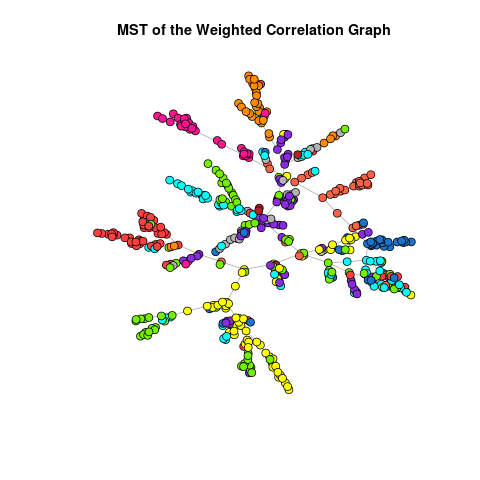
\includegraphics{Figures/q5_monday_mst.png}}
\caption{degree distribution of the correlation graph (weekly data)}
\label{fig:Q5}
\end{figure}









\section{Let's Help Santa!}

\subsection{Download the Data}

\subsection{Build Your Graph}

\subsection{Traveling Salesman Problem}


\textcolor{blue}{
    Question 8: Determine what percentage of triangles in the graph (sets
of 3 points on the map) satisfy the triangle inequality. You do not need
to inspect all triangles, you can just estimate by random sampling of
$1000$ triangles.
}

After the random samplings of $1000$ triangles on the graph, the percentage of triangles in the graph is $93.9\%$.


\textcolor{blue}{
    Question 9: Find the empirical performance of the approximate algorithm:
    \begin{align}
    \rho=\frac{\text{Approximate TSP Cost}}{\text{Optimal TSP Cost}}
    \end{align}
}

According to the $2$-approximate algorithm analysis, we know
\begin{align}
\rho=\frac{\text{Approximate TSP Cost}}{\text{Optimal TSP Cost}}\le 1.5698
\end{align}


\textcolor{blue}{
    Question 10: Plot the trajectory that Santa has to travel!
}

After implementing the $2$-approximate algorithm, the trajectory that Santa has to travel is shown in Fig. \ref{fig:tour}.


\begin{figure}[t]
\centering
\scalebox{1}{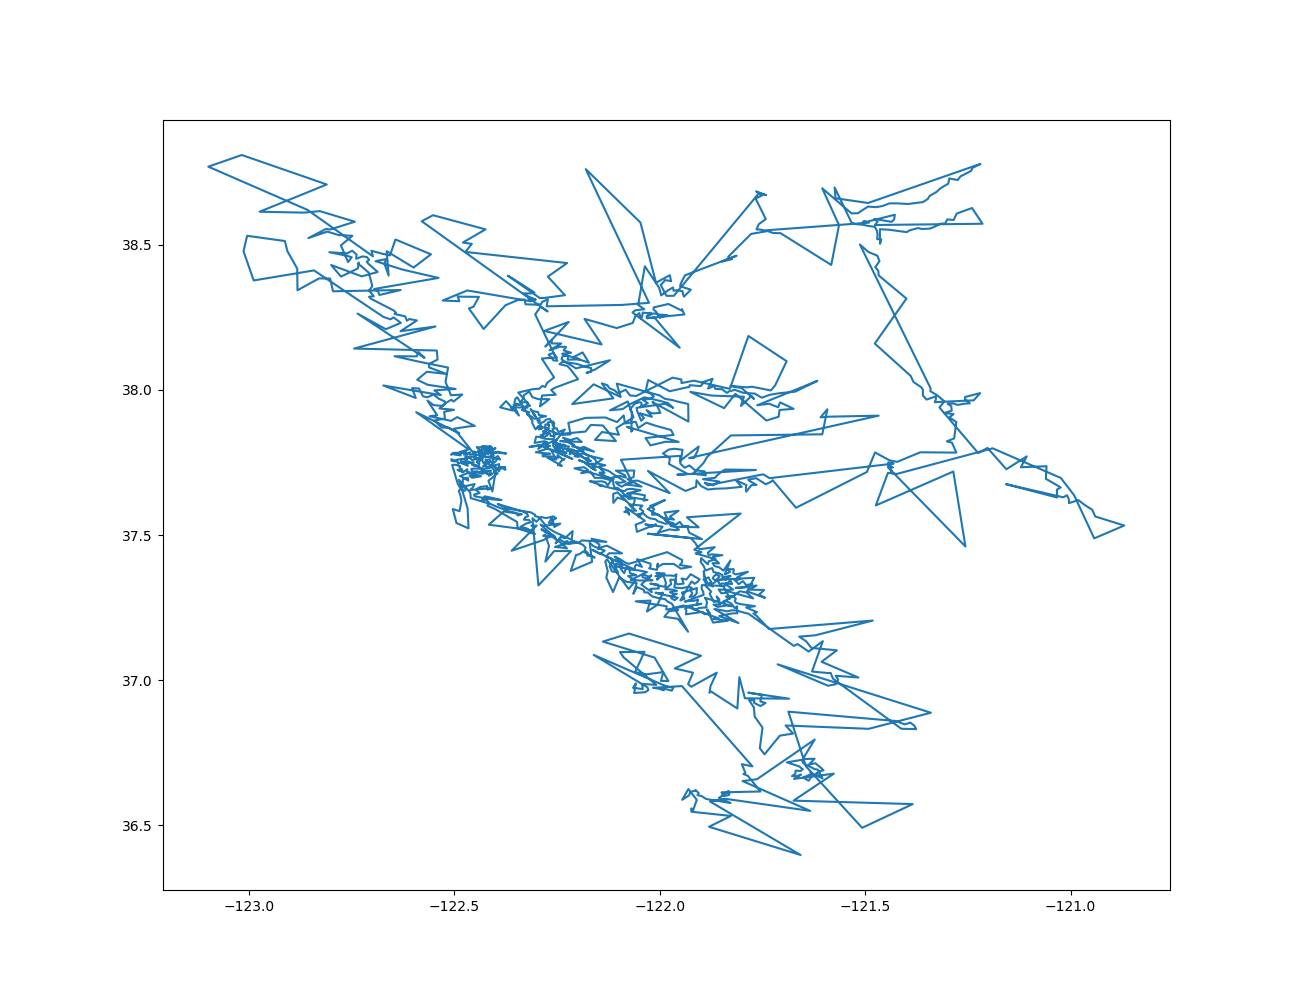
\includegraphics{Figures/tour.png}}
\caption{Travel trajectory that Santa has to travel}
\label{fig:tour}
\end{figure}





\section{Analysing the Traffic Flow}

\subsection{Estimate the Roads}
\textcolor{blue}{
    Question 11: Plot the road mesh that you obtain and explain the result.
Create a subgraph $G_{\Delta}$ induced by the edges produced by triangulation.
}
\begin{figure}[t]
\centering
\scalebox{0.8}{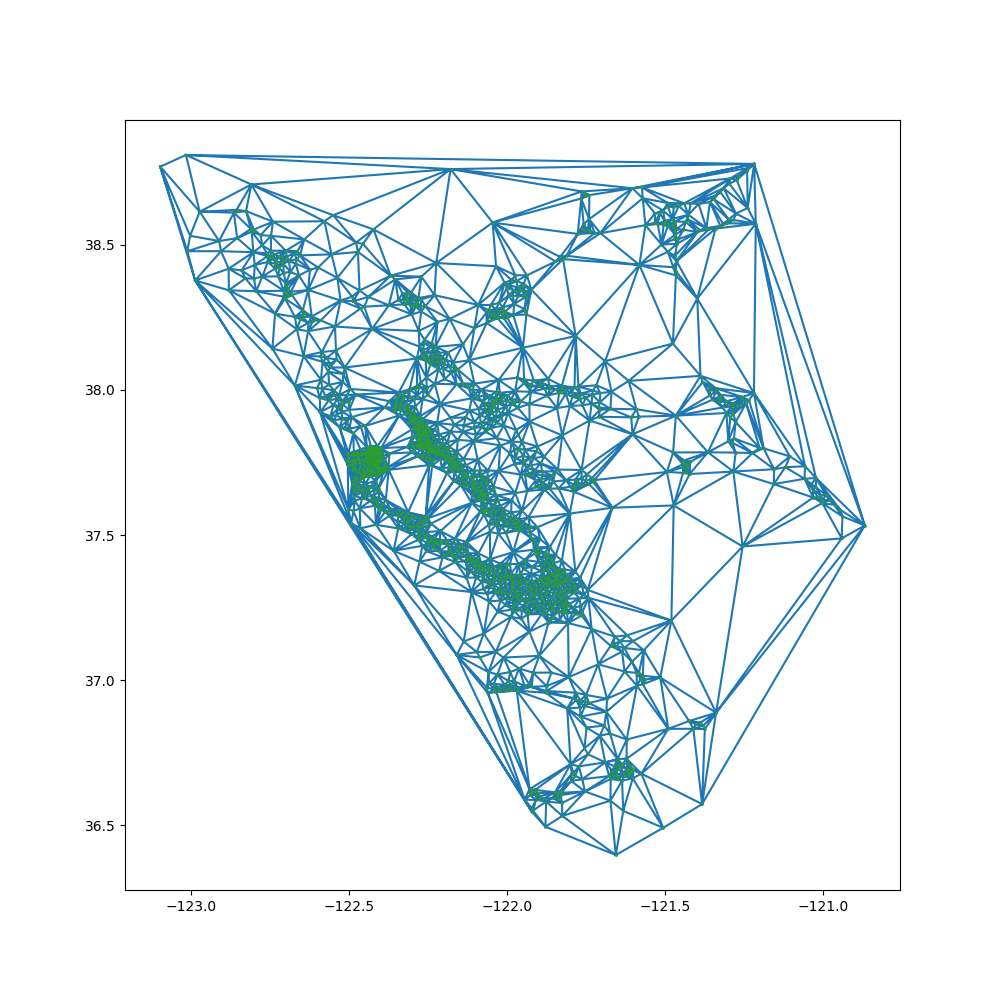
\includegraphics{Figures/triangulation.png}}
\caption{Road mesh after triangulation}
\label{fig:road_mesh}
\end{figure}

After implementing the Delaunay triangulation, the road mesh we obtained is in Fig. \ref{fig:road_mesh}. The road mesh is very similar to the actual map since more dots are needed to characterize the places with high transportation density. On the contrary, only a few number of dots are needed to characterize the wild areas. 



\subsection{Calculate Road Traffic Flows}

\subsection{Calculate the Max Flow}

\subsection{Defoliate Your Graph}













\end{document}
